% This is samplepaper.tex, a sample chapter demonstrating the
% LLNCS macro package for Springer Computer Science proceedings;;
% Version 2.20 of 2017/10/04
%
\documentclass[runningheads]{llncs}
%
\usepackage{graphicx}
% Used for displaying a sample figure. If possible, figure files should
% be included in EPS format..
%
% If you use the hyperref package, please uncomment the following line
% to display URLs in blue roman font according to Springer's eBook style:
% \renewcommand\UrlFont{\color{blue}\rmfamily}

\begin{document}
%
\title{NeoMycelia: A software reference architecture for big data systems}
%
%\titlerunning{Abbreviated paper title}
% If the paper title is too long for the running head, you can set
% an abbreviated paper title here.
%
\author{Pouya Ataei\inst{1}\orcidID{0000-0002-0993-3574} \and
    Alan Litchfield\inst{1}\orcidID{0000-0002-3876-0940}}
%
% \authorrunning{P. Ataei et al.} - no author required
% First names are abbreviated in the running head.
% If there are more than two authors, 'et al.' is used.
%
\institute{Auckland University of Technology, Auckland 1010, New Zealand
    \email{\{pataei, alan.litchfield\}@aut.ac.nz}
}

\maketitle              % typeset the header of the contribution
%
\begin{abstract}
    The big data revolution began when the volume, velocity, and variety of data completely overwhelmed the systems used to store, manipulate and analyze that data. As a result, a new class of software systems emerged called big data systems. While many attempted to harness the power of these new systems, it is estimated that approximately 75\% of the big data projects have failed within the last decade. One of the root causes of this is software engineering and architecture aspect of these systems. This paper aims to facilitate big data system development by introducing a software reference architecture. The work provides an event driven microservices architecture that addresses specific limitations in current big data reference architectures (RA). The artefact development has followed the principles of empirically grounded RAs. The RA has been evaluated by developing a prototype that solves a real-world problem in practice. At the end, succesful implementation of the reference architecture have been presented. The results displayed a good degree of applicability with respect to quality factors.

    \keywords{Reference architecture \and Architecture \and Big data reference architecture \and Big data architecture \and Big data systems \and Big data software engineering \and Event driven \and Microservices}
\end{abstract}
%
%
%
\section{Introduction}
The ubiquity of digital devices, the networking infrastructure of today, and the proliferation of software applications, have augmented users’ capability to produce data at an unprecedented rate \cite{AtaeiHype}. In a world where we have an average processing power of 1.5 GHz on smart phones, and up to 8 GHz on laptops running on a network infrastructure that will support up to 25 Mbps of transmission per second, data becomes the new oil, the atom, the dot that lays the foundation of a nexus \cite{Shafi}.

Big data (BD) is a term that was initially coined to refer to the gradual growth and availability of data \cite{lycett2013datafication}. BD is an endeavor to harness patterns behind vast amounts of data for the purposes of improvement, control, and prediction. Roughly 10 years ago, the BD revolution began when the volume, velocity, and variety of data completely overwhelmed the systems used to store, manipulate and analyze that data \cite{heudecker2014survey,AtaeiBigDataEnvirons}. The concept of BD is a game-changing innovation \cite{chen2017big}, heralds the dawn of a new industrial revolution \cite{Huberty}, and creates a new category of economic asset.

Nevertheless, BD is not always better data or a magic wand that enchants any business or process. Actually, it can very easily cause losses \cite{Ranjan}. It is estimated that approximately 75\% of the BD projects have failed within the last decade according to multiple sources \cite{Partners,analytics2016age,Nash,heudecker2014survey}. Among challenges of adopting BD, the most repeatedly discussed are 1) Architectural and system development challenges, 2) Organizational challenges, and 3) Rapid technology change \cite{chen2017big,AtaeiHype,Singh}. The focus of this study is on architectural and system development challenges.

Today, most BD systems are developed as ad-hoc and complicated architectural solutions that do not tend to adhere to many principles of software engineering \cite{Gorton,Nadal}. In addition, as the ecosystem of BD grows and new technologies are introduced, architects will have harder time to select and orchestrate the right technology to produce the right results \cite{Nadal}.

This can create a foundation for an immature architectural decision that results in a solution that is hard to maintain, hard to scale, and may raise high-entry barriers.  Since the approach of ad-hoc design for BD systems is undesirable and leaves many engineers in the dark, novel software engineering approaches specialized for BD systems are required. To contribute towards this goal, we explore the notion of RAs and present a software reference architecture, Neomycelia.

In the case of ambiguity towards what should be developed to address what needs, RA can play an overarching role to describe the building blocks of the system and the ways in which these blocks communicate to achieve the overall goal of the system \cite{Sievi-Korte}. This in turn produces manageable modules that each address a different aspect of the problem, and provides stakeholders with a high-level medium to observe, reflect upon, communicate with and add into.


\section{Why Reference Architectures?}

BD is an interplay of analytics methods, software engineering through development and data engineering, and organizational workflows \cite{Mannering,Selamat}. Such complex systems are best approached through the lens of architecture and well-thought out design documents. Utilization of RAs for complex systems is not something new.

In fact, practitioners of complex systems, software engineers, and system designers have been frequently using reference architectures to have a collective understanding of system components, functionalities, data-flows and patterns which shape the overall qualities of system and help further adjust it to the business objectives \cite{Kohler,Cloutier}. In software product line (SPL) development, reference architectures are generic schemas that can be configured and instantiated for a particular domain of systems \cite{Derras}. In software engineering, reference architecture (RA) can be defined as means to represent and transfer knowledge that bridges from the problem domain to a family of solutions \cite{Klein}.

RAs serve as a mechanism that embodies domain relevant qualities and concepts, breaks down the solutions and generates a terminology to facilitate effective communication, and illuminates various stakeholders and system designers \cite{Klein}. This allows RAs to provide an opportunity for early identification of design issues, when making changes is still cheap. This has several side-benefits such as: 1) Ensuring cross-cutting concerns are addressed, 2) Scales the knowledge of architects and engineers across the organization, 3) Helps achieving consensus around major design choices, 4) Creates the foundation of organization memory around design decisions, 5) Acts as a blueprint and a summary artefact in the portfolio of the architects and software engineers

% Many of the prevalent technologies in the industry have stemmed from a RA \cite{Cioroaica}. OATH is a commonly used protocol for authentication over the web and the OATH RA is the result of an industry-wide collaboration using open standards \cite{OATH}. Similarly, the ANSI-SPARC architecture, based on the ANSI-SPARC design standard for database management systems \cite{ANSI}, grew to become common among practitioners.


\section{Research Methodology}


To increase systematicity and allow for reproducibility of Neomycelia, we follow the guidelines presented in empirically-grounded RAs \cite{GALSTER}. In essence, “empirically grounded” implies two major aspects: 1) “empirical foundation” which implies that Neomycelia must be grounded in proven principles (domain problems, practical concepts), and 2) “empirical validity” which implies that RA needs to be evaluated for applicability and validity. This research methodology is based on two main pillars: 1) existing RAs and 2) literature on RAs. The process follows these 6 steps:

\textbf{1. Decision on type of the RA}:  A classification framework presented by Angelov et al (\cite{angelov2009classification}) is applied. In this study, five types of RAs have been described from which our RA matches type five (facilitation architectures designed to be implemented in multiple organizations). Thus, this RA aims to facilitate the design of BD systems across multiple organizations. Examples of similar RAs are ERA \cite{angelov2008contracting}, AHA \cite{Wu}, and eSRA \cite{norta2014reference}

\textbf{2. Design Strategy}: There are two general approaches to the development of RAs; developing RAs from scratch or from existing architectures. Our RA is developed based on existing architectures and available literature.

\textbf{3. Empirical acquisition of data}: Data acquisition consists of two major phases, data sources identification and capturing architecture data. It is proposed by Nakagawa et al (\cite{Nakagawa}) that good data sources for classical RA development can be people (researchers, practitioners), available literature (publications, technical reports, white papers) and systems (source codes, documentations). Howbeit, the guidelines presented by Galster and Avgeriou (\cite{GALSTER}), provide no means or instructions on how these data should be identified and captured.

Therefore, to increase systematicity and transparency of this research, we conducted a systematic literature review (SLR) to capture current best evidence from the available literature. For this purpose we follow the guidelines of PRISMA presented by Shamseer et al. (\cite{Shamseer}).

Our aim was to find all available BD reference architectures in literature and gray literature. This has helped by grounding a solid formation for development of Neomycelia. We’ve selected IEEE Explore, ScienceDirect, SpringerLink, ACM library, MIS Quarterly, Elsevier, AISel as well as citation databases such as Scopus, Web of Science, Google Scholar, and Research Gate. The search keywords used are 'Big Data Reference Architectures', 'Reference Architectures in the domain of Big Data', and 'Reference Architectures and Big Data';

In the first phase of the SLR (identification), 84 literature has been pooled. Out of this pool, 57 study has been selected based on our inclusion, exclusion and quality criteria. Studied that provided with detailed analysis and practice have been included. Studied that provided with substantial case studies have been included. Papers that discussed current BD RAs, it’s ecosystems and drivers have been included. Papers that are recent (in the range of 2010-2020) have been included.

On the other hand, papers that are duplicates, do not directly address the SLR aim, and are not written in English are excluded. For our quality factors, we paid extensive attention to how rich the study is in terms of its case studies and relevance to practice. The length and volume of the information provided by the studies has been considered as well. Very short and information lacking papers did not get pass through the quality assessment framework.

In the pool of selected articles, 24.5\% are from SpringerLink, 16\% are from ACM, 33\% are from IEEE Explore, 5.2\% are from ScienceDirect, and the rest are from Google Scholar. 13 conference proceedings, 30 journal articles, 12 book chapters, and a whitepaper has been selected. 33\% belonged to years 2013-2015, 51\% of the articles were selected from the years 2016-2020, and the rest to years 2010-2013.

We used the software Nvivo for classifying and coding the literature. We defined 3 nodes namely ‘big data architecture data’, ‘big data reference architecture limitations’, and ‘big data components”. Once we coded and attributed texts to our nodes, we then synthesized and inferred findings.

The result of this SLR administered 23 RAs from extant literature, 18 RAs from academia, 4 from practice, 1 through the collaboration of both domains. Majority of the RAs have been in the form of short papers, but there has been few detailed RAs as well. The exact detail and listing of the RAs are out of the scope of this study, however, there will be mentions to various RAs for comparison, inference purposes.

We found three common components among all RAs which are; BD management and storage nodes (relational, non-relational, graph, data lake, data finery, polyglot persistence), BD infrastructure nodes (latency, data transformation, in-memory data grids), and BD analytics and application nodes (real-time processing, batch processing, predictive analysis, spatial analysis). This underpinned our understanding for actual design and construction of the RA.

\textbf{4. Construction of the RA}: Based on the findings captured in previous step, the initial design of the RA took place. Integral to this phase, was the underlying method to creation and design of RA. We followed ISO/IEC 42010 for architectural descriptions \cite{Chaabane}. The standard mostly revolves around concrete architectures and because of that, our descriptions do not 100\% conform to it.

For instance, the standard has bolded the identification of system stakeholders (clause 5), however RAs are highly abstract and do not have a clear group of stakeholders \cite{AtaeiACIS}. Another focal point in conveyance of architectural descriptions is the concept of views. In this case, ISO/IEC 42010, being the standard for concrete architectures, prescribe architecture views and viewpoints in the context of business and actual models (clause 4). This does not apply to this RA as well.

Moreover, Beneken et al (\cite{Beneken}) classified three different kind of RAs based on the views, namely functional, logical and technical. Along the lines, Vogel et al. \cite{Vogel} classified RAs based on their usage context, as platform-specific, industry specific, industry crosscutting, and product line RAs.

Whereas different academic efforts aimed at classifying RAs based on different criteria, arguably several distinct views can adhere to one logical view as it has been seen in the case of pattern based reference architecture for serviced based system conducted by Stricker et al. (\cite{Stricker}). This implies, that modules defined in technical review can potentially refine the modules of the logical view. Furthermore, Cloutier et al. (\cite{Cloutier}) suggests that a RA should address business, technical and customer context’s views.

For the purposes of this study we do not address the business view of the RA, as this software RA aims at describing a functional, technical and logical views of a BD system. Business views and viewpoints can be developed later when detailed architectures are needed (Galster and Avgeriou 2011).
After deciding on views and methods of describing architecture, and by analyzing the limitations of current RAs and by in-depth studies of the BD systems, the construction of the RA took place.

\textbf{5. Enable RA with variability}: To allow for easier creation of concrete architectures from this RA, variability has been enabled for some modules. Based on the guidelines of Galster and Avgeriou (\cite{GALSTER}), there are two ways to enable variability: 1) variability models and 2) annotation of the RA. We chose the latter.

\textbf{6. Evaluation of the RA}: Quality of the RA is determined based on two factors: 1) utility and correctness of the RA and 2) the support for instantiation and adoption of the RA \cite{GALSTER}. To achieve these factors, we have created a prototype of the RA and tested it in practice to solve a business problem. Nevertheless, because the RA has not been built from scratch, and has absorbed patterns and principles from existing RAs architectures, and systems in practice, the focus of the evaluation was more towards sufficient support for effective instantiation.


\section{A microservices event-driven reference architecture for big data systems}

In the first iteration of the research methodology discussed in previous section, in step 3, we have captured architectural data and studied common themes in current BD systems. This has laid the foundation of Neomycelia and has illuminated us on the architectural requirements of BD systems. Thus, before the actual design and creation of the software RA, we have first listed the principal characteristics of BD systems and how they should be incorporated into the final artefact.

We have then introduced some of the well-known industrial patterns into the reference architecture and justified it. In what follows, we first discuss the principal characteristics of BD, we then discuss microservices and event driven approaches and justify it. From there on, we will represent the software RA and describe the building blocks.

\subsection{Big data system characteristics}

BD has five principal characteristics: Volume, variety, velocity, veracity, and variability \cite{Nadal,AtaeiHype}. Volume refers to the amount of data passing through various pipelines. In a traditional setup, a data analyst might typically import a fragment of a data warehouse into specialized software for statistical analysis \cite{Ordonez} but this approach is often difficult to achieve with BD deployments. Velocity is the pace at which data flows into the system and gets processed. Commonly through data streams and, to effectively handle arrival irregularities, sliding windows \cite{Babcock}. Variety describes the heterogeneity of data formats. Data often arrives in various formats; structured, semi-structured, or pseudo-structured \cite{Terrizzano,AtaeiBigDataEnvirons}.

Suitable architectural constructs must be created to address variety by, for example, normalizing or reformatting. Veracity refers to data quality, ensured by adherence to data governance protocols \cite{Plotkin}. Data provenance, data quality assessment, data cleansing, and data liveliness are some of the architectural factors that must be taken into consideration. Variability takes into account the evolving nature of data and how data are ingested, processed, and conveyed to the next node in the pipeline \cite{Nadal}. Therefore, Neomycelia must provide:

\begin{itemize}
    \item \textbf{Volume}: Capability of ingesting for massive data sets
    \item \textbf{Velocity}: Enable ingesting from multiple data sources at different rates (scale to demand). It shall support batch-mode and live-stream processing.
    \item \textbf{Variety}: Provide the means for rational processing across different data formats (structured, semi-structured, pseudo-structured)
    \item \textbf{Veracity}: Ensure data quality standards are maintained and includes data provenance, quality, liveliness, and cleansing
    \item \textbf{Variability}: Provide schema evaluation and effective interconnection
\end{itemize}

Taking the innate characteristics of BD into consideration, one should pay clear attention to quality attributes (Cloutier et al. 2010). Quality attributes help identify architectural requirements and key drives.

% and these requirements in turn result in appropriate patterns and tactics.

For the purposes of this software RA, the main quality attributes chosen are modularity, extendibility, modifiability, scalability, maintainability and debuggability.

% These attributes are achieved through a decentralized and distributed approach called event-driven microservices.

\subsection{From monolith to microservices}
Recent approaches to software architecture tends towards increases in modularity and clearly defined boundaries \cite{Jamshidi}. The benefits derived of this shift sees organizations moving to design architectures as series of inter-communicating, yet independent services. Benefits include lower maintenance costs, increased ownership, more agile development, and better support for DevOps, versioning, and scaling \cite{Fritzsch}

Most legacy systems today run on some kind of monolithic architecture. As monolithic applications grow, complexity and overheads increase, making maintenance a daunting task. Adopting new technologies in monolithic systems is difficult and if there exist design changes, the development team may need to put an immense amount of effort to meet new requirements.

In addition, many monolithic systems are not integrated with recent cloud technologies and DevOps trends, for example introducing change or modification to an existing module is prone to side-effects and hard-to-find bugs \cite{Bass,Fritzsch}. Teams are not hundred percent autonomous and holocracy, if it has been adopted, is compromised.

Most RAs and architectural patterns considered for this study have been designed with no attention to microservices. For instance, Lambda (\cite{Villari}) addresses speed, batches, and serving layers. The serving layer addresses the volume characteristics of BD by storing large amounts of heterogonous data in the master dataset.Velocity is addressed by having two different approaches to data processing, speed, and batch processing. While the speed layer usually deals with streams of data that need to be processed in real-time, the batch layer forwards data to the serving layer, and then batch views to allow query processing. Bolster \cite{Nadal} augments this architecture by adding a semantic layer which supports metadata.

Meanwhile, the NIST BD RA \cite{Chang} is the most comprehensive BD RA found in the SLR. The RA is delineated in terms of fabrics, providers, and services. Withall, we could not identify the notion of independent services or clearly defined contexts for the services. Along the lines, there is the pattern based approach conducted by Stricker et al. (\cite{Stricker}) that is heavily inspired by the works of Gamma et al (\cite{Gamma}).

\subsection{The microservices challenge}

Whereas a microservices architecture offers a promising solution to issues related to monolithic systems, the implementation of it can be challenging.
Sometimes referred to as a consequence of ‘monolithic microservices’, one of the key challenges of a successful microservices architecture is effective communication between services \cite{Munaf}.

The basic approach to asynchronous communication is through REST calls, where a service makes a REST call to another service. This is referred to as point-to-point communication and is useful for cases where no response is required or when an admin task needs to be executed. But as services grow, the need for inter-communication increases and if one service is in a blocking state (for example, running a time consuming process), a ripple effect through the whole system is created.

Another approach to asynchronous messaging in a microservices architecture is the publisher-subscriber (pub-sub) model. In this model, a central pub-sub construct (usually a message broker) sits at the heart of the architecture and facilitates communications. This means that, instead of microservices directly calling each other, they publish a new message to the message broker on a specific topic and all the subscribers to that topic will be notified.

Any computational effort is then handled by the subscribers. Furthermore, a subscriber can be a publisher of message too \cite{Indrasiri}. In this case, the message broker is at the heart of the communications process.

\subsection{An event driven approach}

The approaches to microservices communication described require some sort of coupling. Thus, interfaces need to be declared, services need to know what other services are responsible for, how messages will be processed, and services may have dependencies related to other microservices. As microservices increase in number, the maintenance of microservice coupling becomes increasingly challenging.

However, we assert that the concerns above are not the aim of a microservices architecture. Instead, an event driven model provides an effective means of addressing those issues. Point-to-point or pub-sub communication between microservices means that each service should recognise related interfaces and the requirements for downstream microservices \cite{Gupta,Molina}.

The underlying mechanism of existing models is to issue a ‘command’, where one microservice sends commands to another microservice or topic.We provide a ‘dispatch and forget’ approach, in which a service dispatches an event to a central event backbone \cite{Michelson}.

In this way, services do not need to know what happens after an event has been dispatched, they are only responsible for event dispatching through well-defined contracts. The underlying mechanism of this model is ‘event’. Thus, new services can be added, removed, configured, and scaled easily and more simply.

The subtlety lies in the underlying approach, and philosophy of ‘event’ instead of ‘command’, which implies that modules react to a change of state rather than a command for action from another module. This approach solves the issue of long-running tasks that block and a service does not need to wait for another to complete its process.


\section{Neomycelia}
In this section, Neomycelia is described. Strong points for Neomycelia are its attention to metadata and data caching. With the exception of Bolster \cite{Nadal}, RAs scarcely include metadata. Metadata addresses a wide range of needs like security, privacy, scalability, and efficiency. In the context of  a distributed system, metadata bridges data stored in different functions such as in the Cloud versus that on premise \cite{Eichler}.

Furthermore, there was no evidence of an RA that provides for data caching. Avoiding issues related to monolithic systems, and by adhering to principles of event-driven communications, the Neomycelia RA (\ref{NeomyceliaFig}) provides improved modularity, extendibility, modifiability, scalability, and maintainability. This is in line with quality attributes that has been set for evaluation purposes.


\begin{figure}
    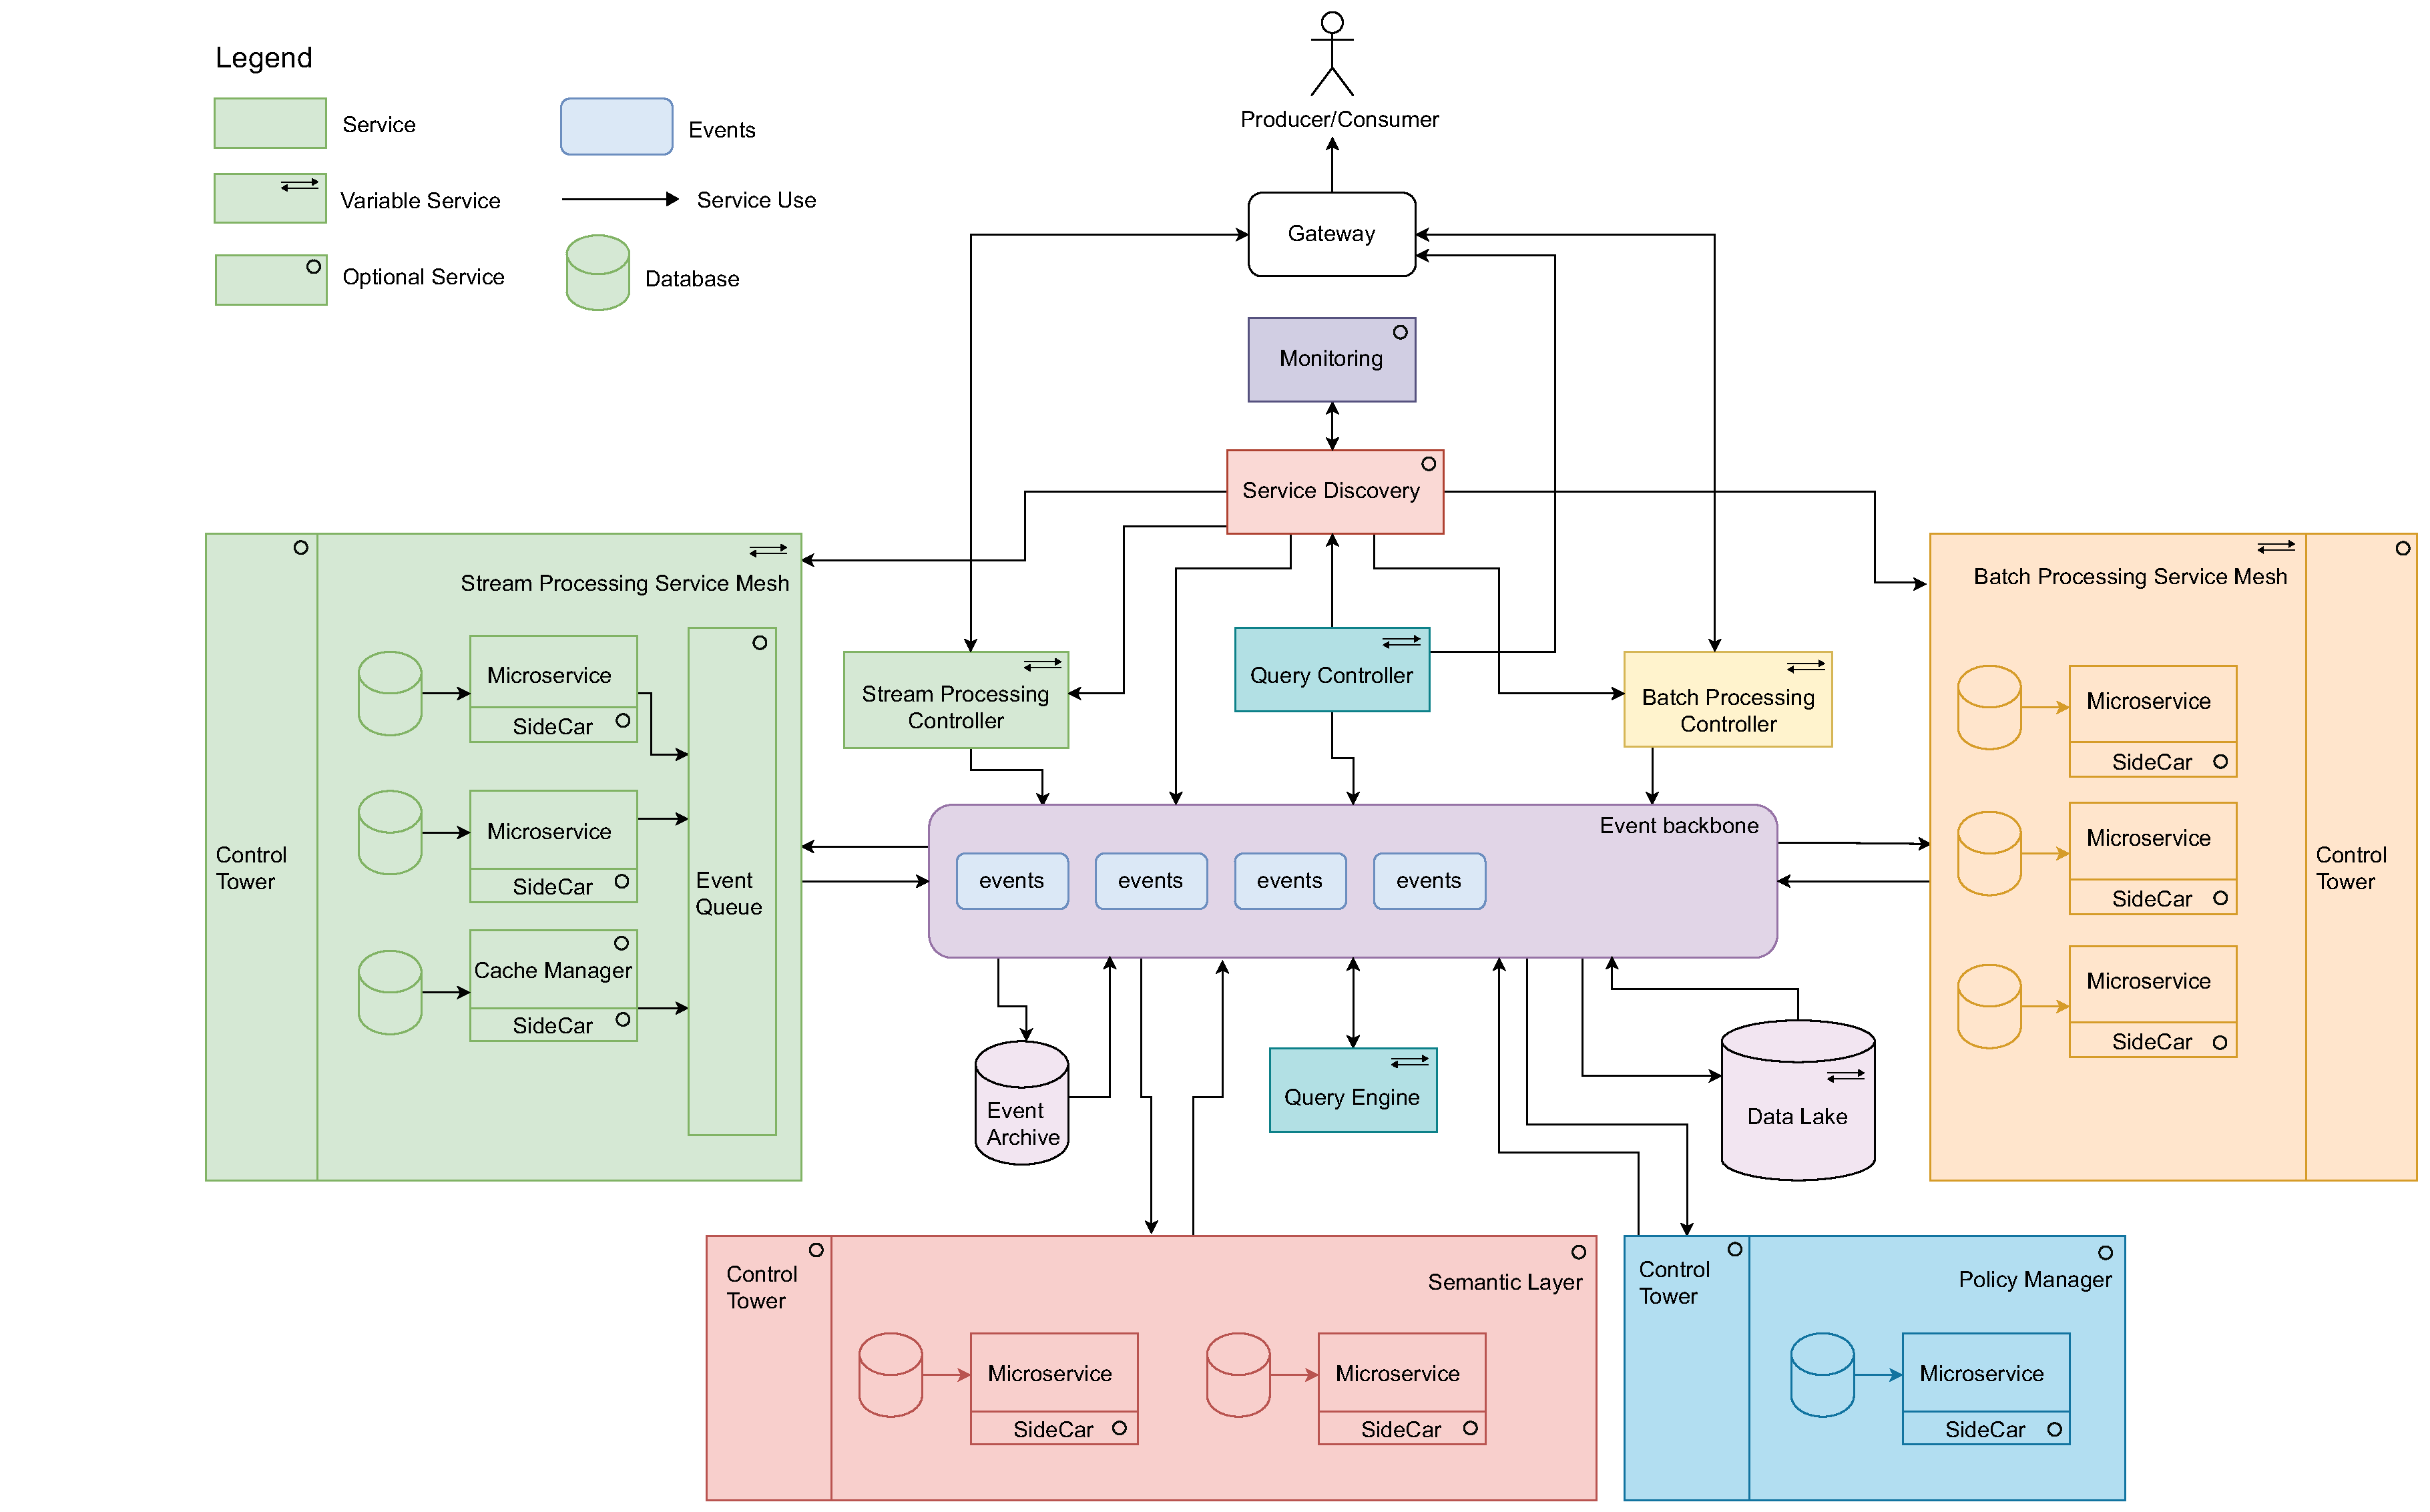
\includegraphics[width=\textwidth]{Neomycelia.eps}
    \caption{Neomycelia Software Reference Architecture.} \label{NeomyceliaFig}
\end{figure}

\subsection{Components}

Neomycelia is comprised of 14 essential architectural components. The terms node, and service are used interchangeably.

\textbf{Gateway}: This is the main entry point and determines how messages are handled. Gateway acts as a reverse proxy that accepts all incoming requests from Application Programming Interfaces (API) and appoints them to appropriate services. This mechanism provides the security, scalability, and maintainability aspects of the RA.

\textbf{Stream processing controller}: This service forwards requests to the stream processing service mesh. Low impact processes like basic sanitization, authentication, and potential validation take place here. Computationally expensive events are not processed in this node. The stream processing controller provides stream provenance and may decide which one-pass algorithm should run over what event stream.

\textbf{Batch processing controller}: The function of this node is to forward requests to the batch processing service mesh. Low impact pre-processing such as preliminary normalization can take please in this node. It is necessary to avoid computationally expensive processes in this service.

\textbf{Stream processing service mesh}: Based on the requirements for specific stream processing approaches, this service is comprised of an arbitrary number of nodes for stream processing. A cache manager keeps track of values processes in the event queue and keeps an event archive with a list of associated computed values. Each service has its own local database. Most stream processing algorithms are operating on in-memory stateful data structures, such as HyperLogLog, to compute distinct values and provide summary output. Different services can adopt unique processing and windowing approaches such as micro-batch processing and tuple-at-a-time \cite{Sahal}.

To avoid obfuscation of the event backbone, each service in the service mesh will communicate its results through an internal message broker (an event queue) that is responsible for communication to the external entities. Linking service results to a message broker that communicate with the event backbone provides parallelism, encapsulates stream processing to its own service mesh, and provides abstraction.

Any service may have a sidecar, or service proxy, attached to it. These proxies act as an intermediary to encapsulate networking and infrastructure needs of the service. Sidecars abstract out all the platform requirements necessary for the service to run. This allows software engineers to focus on what matters, development, and avoid being distracted by infrastructure issues.

Finally, every service mesh will have a control tower which communicates with sidecars and acts as a centralized unit that registers, updates, and passes changes to the services through their proxy. For example, if all services in this service mesh need to update their SSL certificate monthly, they can do it through sidecar communication to the control tower.

\textbf{Batch processing service mesh}: Similar to the stream processing service mesh, except that this does not require a message broker (event queue). Batch processes do not need to happen in real-time, so there is no advantage in providing parallelism. Every service can dispatch directly to the event backbone.

\textbf{Service discovery}: As the number of services increases and deployment and configuration demands become more frequent, identification and invocation of appropriate services become daunting. Service discovery addresses this problem by being a central register for all services. This means, services can now utilize a central node to register their functionalities.

\textbf{Monitoring}: A challenge for a microservices architecture is the ability to track, monitor, and log services behaviors. An event is dispatched from a service, which invokes another service, which in turn results in another dispatch. It’s a difficult task to identify errors in this chain with loosely coupled services but the monitoring service solves this problem by tracking usage and behavioral data from services. Data collection is provided by the service discovery unit. The architect and system designer decide on the granularity of data collected from each service and log aggregation mechanisms.

\textbf{Event backbone}: This is the heart of Neomycelia, facilitating communication between the parts of the system. Every service in the system communicates through event backbone as choreographed events, analogous to a dance troupe where everyone responds to the rhythm of the music and moves according to their specific role. Each service (dancer) listens to the event backbone (the music) and takes action only as required. Thus, a service is responsible only for dispatching an event in a ‘dispatch and forget’ model. Services listening on a specific topic execute the desired process and may dispatch another event to the event backbone.

The event backbone is the sole controller of communication between services, through events. This allows development teams to focus on various services and develop independently. This also allows for simple plug-in and plug-out of a service, reducing concerns about side-effects. Moreover, a failure in a microservice is less likely to affect the whole system because the loss of availability is periodically checked and prevented.

\textbf{Event archive}: Communications between services can sometimes be faulty. Services can timeout, there could be issues in the message contract, the existence of bugs, or type problems. One way to achieve an effective failure handling and recovery approach is through an event archive. This means, if an event fails, it can be retried and recovered because it was registered in an event archive. Furthermore, in the case of an event backbone service going down during an event transmission, the event backbone can recover itself by reading the events it had to handle from the event archive. This can be series of events or a single event.

\textbf{Data Lake}: This contains structured, pseudo-structured, unstructured, and semi-structured data. In a generic setup, data is usually stored in the data lake before it is stream or batch processed. This may not provide the best-case scenario for all situations, so it is up to the architect to decide if that is the most appropriate  data flow in the system.

\textbf{Semantic Layer}: This service mesh is the central hub for all metadata processing, containing the MetaData Management (MDM) system. The MDM is responsible for providing services with information to define and model raw data. This is where a domain vocabulary is defined and controlled by data stewards. The semantic layer provides the opportunity to store metadata, preparation rules, and data evolution and reduces the need for the data analyst or scientist to repeat work. Other semantic practices such as data source register, data transformation log, data cleaning, discretization are also catered for.

\textbf{Policy Manager}: This service mesh is responsible for applying or checking policies about input data. In recent years, data privacy has presented as a challenge in BD management (Bashari Rad et al. 2016), so the policy manager aligns policies with various contexts to determine how data should be retrieved or processed, without significant coupling to the system. As the number of policies increase and are developed, more services can be added to this service mesh. The need for a new policy manager service mesh ought to be rare.

\textbf{Query Controller}: This service determines the type of query received (stream, batch, or other) that come from the gateway and dispatches the event to the query engine. The controller performs straight forward pre-processing or sanitization as required but heavy computation should be avoided.

\textbf{Query Engine}: This service processes query requests. Once values are created, an event is dispatched the subsequent service to return results.

\subsection{Variability}
Neomycelia components are classified as required, variable, and optional. This RA is governed by a strict decoupling rule, such that the removal of any service shall not affect other services.

Gateway, event backbone service, microservices and event archive are required if the architect decides to adhere to the decoupling rule. However, an architect can decide to utilize another method of communication like orchestrated events or point-to-point protocol.The required service gateway provides load balancing, security, lower cumulative latencies, and code simplification. The required service event backbone provides communication between services. The required service event archive is a retry/fail mechanism for the event backbone.

Variable services provided that  a context is maintainable, in which the data lake, stream processing service mesh, batch processing service mesh, controller services (batch, stream, query) and query engine are variable and can be substituted to meet contextual demands.

Optional services include sidecars, control towers, event queue, cache manager services, service discovery service, monitoring service, semantic layer service mesh, and policy manager service mesh. A semantic service mesh and policy manager service mesh provides a solution for privacy and metadata issues in BD systems. An architect may implement a semantic service mesh but must determine if the company cope with the complexity.

\section{Evaluation}

RAs lack clearly defined stakeholders, exist at a high level of abstraction, and are highly adaptable \cite{AtaeiACIS}.RA evaluation is a challenge \cite{angelov2008contracting,Avgeriou,Cioroaica,Maier} because they are not the same as a typical architecture, therefore architecture analysis methods and tools like SAAM (\cite{KazmanSASM}), ALMA (\cite{Bengtsson}), PASA (\cite{Williams}), and ATAM (\cite{KazmanATAM}) cannot be applied. Evaluation of the RA assesses effectiveness, utility, and whether Neomycelia meets its requirements.

This is achieved by evaluating the correctness and utility of the RA, and how efficiently adaptation can be instantiated \cite{GALSTER}. Quality is assessed by how the RA may be transformed into an effective organization-specific concrete architecture. Neomycelia inherits successful attributes from the RAs it is based on. A scenario-based evaluation has been selected that focusses on quality attributes.

Evaluation is being undertaken in an Auckland-based company and being applied to new and existing workflows. The company provides practice management software to veterinary professionals via a Software as a Service (SaaS). The company serves over 15,000 clients from New Zealand, Australia, USA, UK, and Canada with some large equine hospitals and veterinary clinics. ISO/IEC 25000 SQuaRE standard (Software Product Quality Requirements and Evaluation) (\cite{Iso}) is selected as a reference quality model for technology selection. This model is described in terms of characteristics and sub-characteristics.

The explanation of these characteristics is out of the scope of this paper.
Countries adhere to local regulatory frameworks for drug prescriptions for animals, which means local jurisdictions control access to veterinary drugs as Restricted Veterinary Medicines (RVM). Under this protocol, all patients should be background-checked before a drug is dispensed. Therefore, real-time stream processing for background-checks and batch processing for billing triggers and reports generation is needed.  In the future, the system may provide breed detection via image processing of animal photos.

An instantiation of Neomycelia is developed that incorporates Kafka as the event backbone, AWS Lambda for the stream processing and batch processing controllers, Amazon API gateway as the gateway, Envoy for the sidecar services, Kubernetes as cluster manager, Docker for container technology, Resilience4J for a fault-tolerant communication module, Prometheus for the monitoring tool, Zookeeper for the service discovery tool, Istio as the service mesh control tower, Amazon RDS for services private database, Amazon S3 for the event archive, Amazon MQ as the message broker inside the mesh, an Amazon data lake, and Amazon EC2 for services.

A simulation scenario with a request that emulates the system in production has been formulated. While only one topic was created this scenario, adding new topics and services or removing existing ones is fairly trivial. An API gateway has been engineered to pass the request to the representative Lambda. The Lamda performs straightforward preprocessing (adding properties or mutating JSON objects) on the data and dispatches an event to Kafka. In this case, the request needs to be checked against the policies available in that geographic region. Policies are coded in the policy manager services mesh and the controller decides if a request needs to go through a policy manager initially.

The policy manager performs internal processing and decides if a property should be omitted or if the data can even be processed at all. Once done, the policy manager dispatches an event to the relevant topic. If processing is allowed, then the stream processing and batch processing service meshes that are listening for that topic will have their event handlers fired. In the case of batch processing, each service will take the data, process it and then dispatch another event. This is the same for stream processing, with the difference that the requests will go through the message broker first. The controller is also responsible for choosing the storage processing strategy. Whereas most requests are saved in the data lake first, many may need to go through stream processing before that and then be dispatched to the data warehouse.

\section{Conclusion}

As data-oriented technologies emerge, long-established ideologies toward the nature of system design and architecture are revolutionized. Companies are required to be prepared to tackle the apparent difficulty of this field and absorb the complexity. RAs provide a starting point to manage the complexity of BD. In the case of ambiguity towards what should be developed against need, architectures play an overarching role in describing the building blocks of the system and the ways in which blocks communicate to achieve the goals of the system. Future work on Neomycelia and other RAs address security concerns and creating more complex and distributed metadata management technologies.

% ---- Bibliography ----
\bibliographystyle{splncs04}
\bibliography{references}

\end{document}
